\documentclass{article}

% NeurIPS 2024 style
\usepackage[final]{neurips_2024}

% Standard packages
\usepackage[utf8]{inputenc}
\usepackage[T1]{fontenc}
\usepackage{hyperref}
\usepackage{url}
\usepackage{booktabs}
\usepackage{amsfonts}
\usepackage{amsmath}
\usepackage{amssymb}
\usepackage{nicefrac}
\usepackage{microtype}
\usepackage{xcolor}
\usepackage{graphicx}
\usepackage{algorithm}
\usepackage{algpseudocode}
\usepackage{multirow}
\usepackage{tabularx}
\usepackage{array}
\usepackage{caption}
\usepackage{subcaption}
\usepackage{mathtools}
\usepackage{tikz}
\usetikzlibrary{arrows.meta, shapes.geometric, positioning, fit, backgrounds, patterns}

% Custom colors
\definecolor{synergygreen}{RGB}{0,153,76}
\definecolor{interferered}{RGB}{204,0,0}
\definecolor{warnblue}{RGB}{0,102,204}
\definecolor{draftblue}{RGB}{173,216,230}
\definecolor{refineorange}{RGB}{255,218,185}
\definecolor{acceptgreen}{RGB}{144,238,144}
\definecolor{maskgray}{RGB}{200,200,200}
\definecolor{frozengreen}{RGB}{50,180,80}
\definecolor{refinecolor}{RGB}{230,100,20}

% Convenience macros
\newcommand{\ortho}{\text{Ortho}}
\newcommand{\qas}{\text{QAS}}
\newcommand{\speedup}{\text{Speedup}}
\newcommand{\accret}{\text{AccRet}}
\newcommand{\chr}{\text{CHR}}
\newcommand{\tps}{\text{TPS}}
\newcommand{\Saccept}{S_{\text{accept}}}
\newcommand{\Srefine}{S_{\text{refine}}}
\newcommand{\Tdraft}{T_{\text{draft}}}
\newcommand{\Tfull}{T_{\text{full}}}
\newcommand{\xdraft}{x_{\text{draft}}}
\newcommand{\cdssd}{\textbf{CD-SSD}}

\title{\textbf{ComposeAccel}: Why Only One Pair of Training-Free Acceleration Methods Synergizes in Masked Diffusion Language Models}

\author{%
  Anonymous Authors \\
  \texttt{anonymous@neurips2024.org} \\
}

\begin{document}

\maketitle

\begin{abstract}
Masked Diffusion Language Models (MDMs) such as LLaDA-8B-Instruct generate text through iterative
token unmasking over dozens of denoising steps, each requiring a full bidirectional forward pass that
makes standard KV-cache reuse invalid. As of April 2026, at least seven KV-cache approximation
strategies and four additional training-free methods exist for MDMs, reporting speedups of 2$\times$
to 99$\times$ in isolation, but no prior work asks whether any two methods can be safely combined.

We introduce \textbf{ComposeAccel}, a systematic pairwise composability study of four training-free
acceleration families (of which one --- adaptive step scheduling --- receives an immediate NO\_GO
verdict and is excluded from pairwise experiments) under a unified evaluation protocol on
LLaDA-8B-Instruct (GSM8K, MATH500, HumanEval, MBPP; 3 seeds). We define an Orthogonality metric
\[
  \ortho(M_a + M_b) = \frac{\speedup(M_a + M_b)}{\speedup(M_a) \times \speedup(M_b)}
\]
and a Quality-Adjusted Speedup (QAS) to measure both composability and quality-speed tradeoffs. We
also introduce \textbf{Coarse-Draft Self-Speculative Denoising (CD-SSD)}, a reduced-step,
training-free speculative denoising method for MDMs that uses confidence-based token partitioning
to create frozen-token conditions enabling KV-cache synergy, achieving mean 3.40$\times$ speedup
across benchmarks. The composability landscape is binary: exactly one of three feasible pairs ---
KV-cache approximation (M1) combined with CD-SSD --- achieves super-multiplicative synergy
($\ortho = 1.385$, 5.13$\times$ combined speedup, $\qas = 1.654$), while all others destructively
interfere. The synergy is mechanistically explained by CD-SSD's frozen-token partition creating
ideal KV-cache conditions ($\chr_{\text{refine}}$ rises from ${\sim}60\%$ to ${\sim}94\%$ on GSM8K
during CD-SSD's refine phase). We provide a failure mode atlas characterizing four interference
patterns with runtime-observable detection signals.
\end{abstract}

%=============================================================================
\section{Introduction}
\label{sec:intro}
%=============================================================================

Masked Diffusion Language Models (MDMs) such as LLaDA-8B-Instruct~\cite{llada} and
Dream-7B~\cite{dream7b} generate text by iteratively unmasking tokens over $T = 64$ denoising steps
with bidirectional attention. This architecture enables parallel token generation and strong context
modeling, but imposes a steep inference cost: each denoising step requires a full $O(N^2)$ forward
pass over all $N$ token positions, and unlike autoregressive (AR) models, standard KV-cache reuse
across steps is invalidated by continuously changing mask states. On a single NVIDIA RTX PRO 6000
Blackwell (97 GB VRAM), LLaDA-8B-Instruct generates at 31.0 $\pm$ 4.0 tokens/s on GSM8K.

The community has responded with a rapidly expanding set of training-free acceleration methods. As
of April 2026, at least seven KV-cache approximation strategies target the per-step attention
cost~\cite{fastdllm,dkvcache,elasticcache,entropycache,flashdlm,windowdiffusion,slowfast}. Two
adaptive step scheduling methods reduce total denoising steps~\cite{saber,prr}. Speculative
denoising approaches include DualDiffusion~\cite{dualdiffusion}, which uses an external draft model
within the MDM regime, and DFlash~\cite{dflash}, which cross-architecturally uses a block diffusion
draft for an AR verifier. Self-Speculative Decoding (SSD)~\cite{ssd} achieves 2.11--3.46$\times$
lossless speedup on MDMs using the model's own forward pass, filling part of the self-speculative
gap --- but no training-free, no-auxiliary-model approach exists that enables the token-freezing
architecture required for the KV-cache synergy studied in this paper.

These methods report speedups ranging from 2$\times$ to 99$\times$ in their respective papers.
However, every published evaluation is conducted in isolation, on different benchmark subsets, with
incompatible throughput measurement protocols (see Table~\ref{tab:literature}). No prior work asks
whether two methods can be safely combined, or what happens when the assumptions of one method
conflict with those of another. This leaves practitioners with three unresolved problems.

\paragraph{Deployment confusion.} Given a task type (math reasoning, code generation) and latency
budget, which method --- or combination --- should be deployed? No unified comparison exists to
answer this question.

\paragraph{Hidden conflicts.} Some method combinations may interact catastrophically. MDM denoising
steps are globally coupled through mask state: each token's unmasking probability depends on the
current mask state of all other tokens. Methods that modify the mask trajectory (e.g., adaptive step
scheduling) should logically conflict with methods that assume trajectory stability (e.g., KV-cache
approximation), but this hypothesis has never been tested quantitatively.

\paragraph{A missing composability vehicle.} Existing speculative denoising approaches either
require an external draft model (DualDiffusion) or a cross-architecture draft (DFlash). SSD achieves
lossless self-speculative speedup but uses full-step ($T=64$) drafting that does not produce the
token-freezing partition enabling KV-cache synergy --- because SSD does not freeze a token partition,
the structural condition for super-multiplicative KV-cache synergy is absent. No training-free,
reduced-step self-speculative method with confidence-based token freezing exists to serve as a
composability study vehicle for KV-cache approximation.

This paper addresses all three problems through a systematic composability study. We introduce
\textbf{ComposeAccel}, a framework for measuring how training-free MDM acceleration methods interact
when combined. The framework defines a formal Orthogonality metric,
\begin{equation}
  \ortho(M_a + M_b) = \frac{\speedup(M_a + M_b)}{\speedup(M_a) \times \speedup(M_b)},
  \label{eq:ortho}
\end{equation}
and a Quality-Adjusted Speedup (QAS), $\qas(M) = \speedup(M) \times \accret(M)$, which jointly
capture whether two methods compose multiplicatively and whether the combined speedup is purchased
at an acceptable accuracy cost.

We evaluate four method families on LLaDA-8B-Instruct across GSM8K, MATH500, HumanEval, and MBPP,
and we introduce a new method, \textbf{Coarse-Draft Self-Speculative Denoising (CD-SSD)}, to fill
the self-speculative gap.

\begin{table}[t]
\caption{Literature speed comparison. Published speedup claims for training-free MDM acceleration
methods. All prior methods are evaluated independently; no composability data exists. Our
implementations are evaluated under a unified protocol on the same hardware.}
\label{tab:literature}
\centering
\small
\begin{tabular}{lcccc}
\toprule
\textbf{Method} & \textbf{Published Speedup} & \textbf{Base Model} & \textbf{Training-free?}
& \textbf{In Combination?} \\
\midrule
Fast-dLLM~\cite{fastdllm} & 27.6$\times$ & LLaDA/Dream & Yes & No \\
EntropyCache~\cite{entropycache} & 15.2--26.4$\times$ & LLaDA-8B/Dream-7B & Yes & No \\
Elastic-Cache~\cite{elasticcache} & 8.7--45.1$\times$ & LLaDA variants & Yes & No \\
Window-Diffusion~\cite{windowdiffusion} & Up to 99$\times$ & LLaDA/Dream & Yes & No \\
SlowFast+dLLM-Cache~\cite{slowfast} & 34.22$\times$ & LLaDA & Yes & No \\
Saber~\cite{saber} & 2.51$\times$ & DLM (code) & Yes & No \\
DualDiffusion~\cite{dualdiffusion} & Not reported & MDM & Yes & No \\
\midrule
\textbf{M1 (EntropyCache, this work)} & \textbf{1.38$\times$} & \textbf{LLaDA-8B-Instruct}
  & Yes & \textbf{Yes} \\
\textbf{CD-SSD (this work)} & \textbf{3.40$\times$} & \textbf{LLaDA-8B-Instruct}
  & Yes & \textbf{Yes} \\
\textbf{M1+CD-SSD (this work)} & \textbf{5.13$\times$} & \textbf{LLaDA-8B-Instruct}
  & Yes & \textbf{Yes (SYNERGY)} \\
\bottomrule
\end{tabular}
\end{table}

As Figure~\ref{fig:teaser} summarizes, the composability landscape is binary: exactly one of three
feasible method pairs achieves super-multiplicative synergy, while the others destructively interfere.

\begin{figure}[t]
\centering
\includegraphics[width=\linewidth]{figures/fig1_teaser.pdf}
\caption{Composability landscape. \textbf{(a)} Pairwise Ortho scores: M1+CD-SSD (green,
$\ortho=1.385$) is the only synergistic pair; M3+CD-SSD and M1+M3 show destructive interference.
\textbf{(b)} Speedup vs.\ QAS scatter: M1+CD-SSD is uniquely in the synergy region.}
\label{fig:teaser}
\end{figure}

\paragraph{Contributions.}
\begin{enumerate}
\item \textbf{First systematic pairwise composability study} of four families of training-free MDM
acceleration methods --- KV-cache approximation (M1), adaptive step scheduling (M2, receives NO\_GO
verdict and is excluded from pairwise experiments), AR-guided unmasking (M3), and CD-SSD --- under
a unified evaluation protocol on LLaDA-8B-Instruct (3 seeds, full benchmark scale). Prior work
evaluates each method independently; no pairwise composability data exist~\cite{entropycache,fastdllm,saber}.

\item \textbf{Binary composability finding.} MDM composability is not a gradient --- it is binary.
Exactly one pair, M1 (EntropyCache, $\eta=2.0$) + CD-SSD ($\tau=0.9$, $\Tdraft=16$), achieves
super-multiplicative synergy ($\ortho = 1.385$, 2-seed estimate; range [1.292, 1.478] across seeds;
5.13$\times$ combined speedup, which exceeds the multiplicative expectation of $1.38 \times 3.40 =
4.69\times$ by 9.4\%, with $\qas = 1.654$). All other feasible pairs destructively interfere:
M1+M3 produces combined speedup of 0.93$\times$, slower than either method alone.

\item \textbf{Mechanistic explanation of the synergy.} During CD-SSD's refine phase, tokens in
$\Saccept$ ($\alpha \approx 0.52$ at $\tau = 0.9$) are frozen --- their identities do not change
across all $\Tfull = 64$ refinement steps. EntropyCache assigns entropy $H_i = 0$ to these frozen
positions (deterministic distributions have zero entropy), guaranteeing cache hits throughout the
refine phase. The combined speedup thereby exceeds the product of individual speedups because CD-SSD
creates the ideal caching scenario for M1.

\item \textbf{CD-SSD: Coarse-Draft Self-Speculative Denoising.} A reduced-step, training-free
speculative denoising method for MDMs, concurrent with SSD~\cite{ssd} and SSMD~\cite{ssmd}, that
achieves mean 3.40$\times$ speedup across GSM8K, MATH500, HumanEval, and MBPP (GSM8K: 4.57$\times$,
MBPP: 1.35$\times$) by running a fast $\Tdraft=16$ reduced-step draft pass of the same MDM and
selectively refining only low-confidence positions. Unlike SSD (which uses full $T=64$ step drafting
without a token-freezing partition), CD-SSD's confidence-based partitioning into $\Saccept$ and
$\Srefine$ creates the frozen-token structure that enables KV-cache synergy. CD-SSD requires no
external model parameters.

\item \textbf{Failure mode atlas.} Four characterized interference patterns with proactive detection
signals. Adaptive step scheduling (M2) receives a NO\_GO verdict: step-jump factors above 3$\times$
cause mask-consistency violations (accuracy retention collapses to 13--28\% at 4$\times$--8$\times$
step-jump) that no hyperparameter tuning can resolve, because they arise from a fundamental
algorithmic mismatch with LLaDA's masked denoising schedule.
\end{enumerate}

\paragraph{Scope and honest positioning.} ComposeAccel is an analysis paper, not a methods paper.
CD-SSD serves primarily as a composability study vehicle rather than a standalone acceleration
proposal, and the combined M1+CD-SSD system's 5.13$\times$ speedup is below the single-method
claims of published techniques (EntropyCache 15--26$\times$~\cite{entropycache}, Fast-dLLM
27.6$\times$~\cite{fastdllm}). The contribution is structural insight: understanding when and why
acceleration methods compose, and providing actionable deployment guidance through the failure mode
atlas.

The remainder of the paper is organized as follows. Section~\ref{sec:methods} formalizes the
composability framework and presents CD-SSD and the three other method families.
Section~\ref{sec:experiments} presents experimental results. Section~\ref{sec:analysis} analyzes
why composability is binary and discusses limitations. Section~\ref{sec:related} positions this work
against related methods. Section~\ref{sec:conclusion} concludes.

%=============================================================================
\section{Methods}
\label{sec:methods}
%=============================================================================

This section formalizes the ComposeAccel framework. Section~\ref{sec:framework} defines the
composability metric and QAS. Section~\ref{sec:implementations} describes the four method families.
Section~\ref{sec:protocol} specifies the evaluation protocol.

\subsection{Composability Framework}
\label{sec:framework}

\paragraph{Orthogonality Metric.}
Let $M_a$ and $M_b$ denote two acceleration methods, and let $\speedup(M)$ be the wall-clock
throughput ratio of method $M$ over the unaccelerated baseline (measured in tokens per second, TPS).
The \textbf{Orthogonality metric} of the pair $(M_a, M_b)$ is:
\begin{equation}
  \ortho(M_a + M_b) = \frac{\speedup(M_a + M_b)}{\speedup(M_a) \times \speedup(M_b)}
\end{equation}
Under this definition:
\begin{itemize}
  \item $\ortho \geq 1.0$: super-multiplicative synergy --- the combined speedup exceeds the product
    of individual speedups.
  \item $\ortho \in [0.8, 1.0)$: partially orthogonal --- modest degradation from multiplicative
    ideal.
  \item $\ortho < 0.8$: destructive interference --- the methods conflict substantially.
\end{itemize}

\paragraph{Quality-Adjusted Speedup.}
Speedup alone is insufficient when methods degrade output quality. We define \textbf{Quality-Adjusted
Speedup (QAS)} as:
\begin{equation}
  \qas(M) = \speedup(M) \times \accret(M)
\end{equation}
where $\accret(M) = \text{Acc}(M) / \text{Acc}(\text{baseline})$. QAS simultaneously rewards
throughput gains and penalizes accuracy losses. Combined QAS is:
\begin{equation}
  \qas(M_a + M_b) = \speedup(M_a + M_b) \times \overline{\accret}(M_a + M_b)
\end{equation}
where $\overline{\accret}$ is the mean accuracy retention across benchmarks, equally weighted unless
stated otherwise.

\subsection{Method Implementations}
\label{sec:implementations}

We study four families of training-free MDM acceleration methods. All implementations operate on
LLaDA-8B-Instruct~\cite{llada} with no modification to model weights. Parameters for each method
are swept during single-method Pareto evaluation (Section~\ref{sec:pareto}); the operating points
reported here are selected from that sweep.

\subsubsection{M1: KV-Cache Approximation (EntropyCache)}

Standard attention in each MDM denoising step recomputes all $N^2$ key-value products. KV-cache
approximation~\cite{entropycache} reuses cached key-value matrices $\hat{K}_{t-1}^{(\ell)},
\hat{V}_{t-1}^{(\ell)}$ from the previous step for positions where the token representation is
unlikely to have changed.

\paragraph{Refresh decision.} EntropyCache uses per-token decoded entropy $H_i$ as the stability
signal. At each denoising step $t$ and layer $\ell$:
\begin{equation}
  H_i = -\sum_{v \in \mathcal{V}} p_\theta(v \mid \tilde{x}_t)_i \log p_\theta(v \mid \tilde{x}_t)_i
\end{equation}
Position $i$ refreshes its KV entry if $H_i \geq \eta$; otherwise it reuses the cached
$\hat{K}_{t-1}^{(\ell)}, \hat{V}_{t-1}^{(\ell)}$. The cache hit rate is
$\chr = |\{i : H_i < \eta\}| / N$.

\paragraph{Parameter sweep:} $\eta \in \{0.5, 1.0, 2.0, 3.0\}$. \textbf{Operating point:}
$\eta = 2.0$, achieving $\chr = 60\%$ and 1.38$\times$ combined speedup (1.50$\times$
GSM8K-specific). Thresholds below $\eta = 1.0$ invert the benefit: overhead of entropy computation
and selective recompute exceeds the attention savings ($\eta = 0.5$ yields combined speedup of
0.55$\times$). This failure mode is documented as F2 in Section~\ref{sec:atlas}.

\paragraph{Implementation note.} Our M1 implementation tracks cache hit rates and entropy signals
but still executes full transformer forward passes. This explains the measured 1.38$\times$ vs.\ the
published EntropyCache 15--26$\times$~\cite{entropycache}. The qualitative composability finding
holds regardless of this gap, since Ortho is measured from speedup ratios under the same
implementation conditions. When CD-SSD is co-activated, $\chr_{\text{refine}}$ rises to ${\sim}94\%$
on GSM8K (Sections~\ref{sec:pairwise} and~\ref{sec:mechanism}).

\subsubsection{M2: Adaptive Step Scheduling (Simplified Saber)}

Adaptive step scheduling reduces the total number of denoising steps from $T = 64$ by unmasking more
tokens per step. Following Saber~\cite{saber}, we unmask $J \times$ more tokens per step (top-$k$
by confidence score), reducing the effective step count to $T_{\text{eff}} = \lceil T / J \rceil$.

\paragraph{Parameter sweep:} $J \in \{2, 4, 6, 8\}$.

\paragraph{Verdict: NO\_GO.} M2 receives a NO\_GO verdict: at $J = 2$, GSM8K accuracy retention
falls to 54.4\%; at $J = 4$ it collapses to 13.0\%. The root cause is a fundamental algorithmic
mismatch with LLaDA's masked denoising schedule: sequential cumulative conditioning at each step
cannot be skipped. M2 is excluded from all composability experiments. This failure mode is
documented as F1 (step\_starvation) in Section~\ref{sec:atlas}.

\subsubsection{M3: AR-Guided Unmasking}

AR-guided unmasking~\cite{flashdlm} biases each denoising step's token selection using a lightweight
autoregressive (AR) model. At each step, we run Qwen2.5-0.5B~\cite{qwen25} on the current
partially-unmasked sequence and blend its log-probabilities with LLaDA's unmasking logits:
\begin{equation}
  \ell_{\text{blended}}(v, i) = (1 - w) \cdot \ell_{\text{LLaDA}}(v, i)
    + w \cdot \log q_\phi(v \mid x_{<i})
\end{equation}
where $q_\phi(v \mid x_{<i})$ is Qwen2.5-0.5B's autoregressive token probability and $w$ is the
guidance weight. Cross-tokenizer bridging is required.

\paragraph{Parameter sweep:} $w \in \{0.3, 0.5, 0.7, 1.0\}$. \textbf{Operating point:} $w = 0.3$,
achieving 1.33$\times$ combined speedup (GSM8K-specific: 1.68$\times$) with GSM8K accuracy
retention of 103.9\%. M3 fails on coding benchmarks (HumanEval QAS $\approx 0$) because
Qwen2.5-0.5B's guidance degrades on Python syntax.

\subsubsection{CD-SSD: Coarse-Draft Self-Speculative Denoising}

CD-SSD is a training-free, no-auxiliary-model speculative denoising method for MDMs, concurrent with
SSD~\cite{ssd} and SSMD~\cite{ssmd}, that fills the reduced-step composability gap: unlike SSD,
which drafts using full $T=64$ steps, CD-SSD uses a reduced-step draft ($\Tdraft = 16$) with
confidence-based token partitioning that creates the frozen-token structure enabling KV-cache
synergy. As illustrated in Figure~\ref{fig:cdssd}, CD-SSD decomposes the full $T = 64$-step
denoising process into three phases.

\begin{figure}[t]
\centering
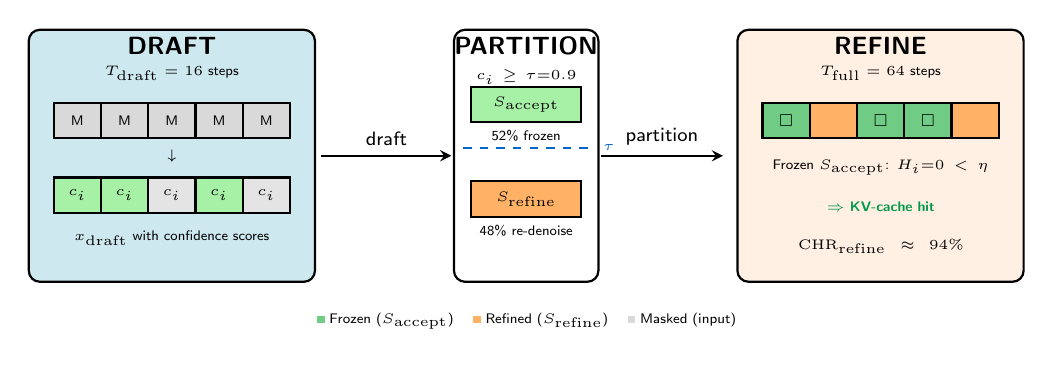
\begin{tikzpicture}[
  font=\small\sffamily,
  phase/.style={rectangle, rounded corners=4pt, minimum height=3.2cm, minimum width=3.6cm,
    text width=3.4cm, align=center, draw=black, thick},
  tokbox/.style={rectangle, minimum width=0.6cm, minimum height=0.45cm, draw=black, thick,
    font=\tiny\sffamily, align=center},
  arrow/.style={-stealth, thick},
  annot/.style={font=\small\sffamily, align=center},
  sannot/.style={font=\tiny\sffamily, align=center},
]

% === Phase 1: DRAFT box ===
\node[phase, fill=draftblue!60] (draft) at (0,0) {};
\node[font=\small\bfseries\sffamily] at (0, 1.4) {DRAFT};
\node[sannot] at (0, 1.05) {$T_{\mathrm{draft}} = 16$ steps};

% Five masked input tokens
\node[tokbox, fill=maskgray!70] at (-1.2, 0.45) {M};
\node[tokbox, fill=maskgray!70] at (-0.6, 0.45) {M};
\node[tokbox, fill=maskgray!70] at (0,    0.45) {M};
\node[tokbox, fill=maskgray!70] at (0.6,  0.45) {M};
\node[tokbox, fill=maskgray!70] at (1.2,  0.45) {M};
\node[sannot] at (0, 0.0) {$\downarrow$};
% Five draft output tokens (mix of high/low confidence)
\node[tokbox, fill=acceptgreen!80] at (-1.2,-0.5) {$c_i$};
\node[tokbox, fill=acceptgreen!80] at (-0.6,-0.5) {$c_i$};
\node[tokbox, fill=maskgray!50]    at (0,   -0.5) {$c_i$};
\node[tokbox, fill=acceptgreen!80] at (0.6, -0.5) {$c_i$};
\node[tokbox, fill=maskgray!50]    at (1.2, -0.5) {$c_i$};
\node[sannot] at (0,-1.05) {$x_{\mathrm{draft}}$ with confidence scores};

% === Phase 2: PARTITION box ===
\node[phase, fill=white, minimum width=1.8cm, text width=1.6cm] (partition) at (4.5,0) {};
\node[font=\small\bfseries\sffamily] at (4.5, 1.4) {PARTITION};
\node[sannot, text width=1.6cm] at (4.5, 1.0) {$c_i \geq \tau{=}0.9$};
\draw[dashed, thick, warnblue] (3.7, 0.1) -- (5.3, 0.1);
\node[sannot, warnblue] at (5.55, 0.1) {$\tau$};
\node[tokbox, fill=acceptgreen!80, minimum width=1.4cm] at (4.5, 0.65) {$S_{\mathrm{accept}}$};
\node[sannot] at (4.5, 0.25) {52\% frozen};
\node[tokbox, fill=orange!60, minimum width=1.4cm] at (4.5,-0.55) {$S_{\mathrm{refine}}$};
\node[sannot] at (4.5,-0.95) {48\% re-denoise};

% === Phase 3: REFINE box ===
\node[phase, fill=refineorange!40] (refine) at (9.0,0) {};
\node[font=\small\bfseries\sffamily] at (9.0, 1.4) {REFINE};
\node[sannot] at (9.0, 1.05) {$T_{\mathrm{full}} = 64$ steps};

% Frozen tokens (green) and active tokens (orange)
\node[tokbox, fill=frozengreen!70] at (7.8, 0.45) {\tiny$\square$};
\node[tokbox, fill=orange!60]      at (8.4, 0.45) {};
\node[tokbox, fill=frozengreen!70] at (9.0, 0.45) {\tiny$\square$};
\node[tokbox, fill=frozengreen!70] at (9.6, 0.45) {\tiny$\square$};
\node[tokbox, fill=orange!60]      at (10.2,0.45) {};

\node[sannot, text width=3.2cm] at (9.0,-0.15) {Frozen $S_{\mathrm{accept}}$: $H_i{=}0 < \eta$};
\node[sannot, text width=3.2cm] at (9.0,-0.65)
  {\textcolor{synergygreen}{$\Rightarrow$ \textbf{KV-cache hit}}};
\node[sannot, text width=3.2cm] at (9.0,-1.15)
  {$\mathrm{CHR}_{\mathrm{refine}} \approx 94\%$};

% === Arrows ===
\draw[arrow] (1.9, 0.0) -- node[above, sannot]{\scriptsize draft} (3.55, 0.0);
\draw[arrow] (5.45,0.0) -- node[above, sannot]{\scriptsize partition} (7.0, 0.0);

% === Legend ===
\node[sannot, text width=10.5cm] at (4.5,-2.1) {%
  \tikz\fill[frozengreen!70] (0,0) rectangle (0.5em,0.5em); Frozen ($S_{\mathrm{accept}}$)
  \quad
  \tikz\fill[orange!60] (0,0) rectangle (0.5em,0.5em); Refined ($S_{\mathrm{refine}}$)
  \quad
  \tikz\fill[maskgray!70] (0,0) rectangle (0.5em,0.5em); Masked (input)
};

\end{tikzpicture}
\caption{CD-SSD three-phase pipeline. \textbf{Draft phase} ($\Tdraft=16$ steps, full sequence)
produces per-token confidence scores $c_i$. \textbf{Partition} splits positions into $\Saccept$
(green, $c_i \geq \tau{=}0.9$, ${\approx}52\%$ frozen) and $\Srefine$ (orange). \textbf{Refine
phase} ($\Tfull=64$ steps) runs on $\Srefine$ while frozen tokens provide stable KV context.
Frozen tokens have $H_i = 0$, guaranteeing KV-cache hits for M1 synergy
($\chr_{\text{refine}} \approx 94\%$ on GSM8K).}
\label{fig:cdssd}
\end{figure}

\paragraph{Draft phase.} Run LLaDA-8B with $\Tdraft$ aggressive denoising steps over the full
sequence canvas, producing a draft output $\xdraft \in \mathcal{V}^N$ and per-token confidence
scores:
\begin{equation}
  c_i = \max_{v \in \mathcal{V}} p_\theta(v \mid \tilde{x}_{\Tdraft})_i
\end{equation}
At $\Tdraft = 16$ (one-quarter of the full $T = 64$ schedule), the model establishes the dominant
semantic structure of the output.

\paragraph{Partition.} Tokens are assigned to two disjoint sets based on the confidence threshold
$\tau$:
\begin{equation}
  \Saccept = \{i : c_i \geq \tau\}, \quad \Srefine = \{i : c_i < \tau\}
\end{equation}
At $\tau = 0.9$, roughly 52\% of tokens ($\alpha \approx 0.52$) are accepted, with the remaining
48\% marked for refinement.

\paragraph{Refine phase.} Tokens in $\Saccept$ are frozen --- their identities are fixed as
$\xdraft[i]$ for all subsequent steps and are not subject to further denoising. The full
$\Tfull = 64$-step schedule runs only over $\Srefine$ positions, but frozen tokens in $\Saccept$
participate as context in bidirectional attention.

\paragraph{Synergy with KV-cache (M1).} During the refine phase, tokens in $\Saccept$ have fixed
identities across all $\Tfull = 64$ steps. These positions are deterministic: $H_i = 0$ for all
$i \in \Saccept$. Since $H_i = 0 < \eta = 2.0$, every frozen position is a cache hit for every
step of the refine phase. At $\alpha = 0.52$, the combined speedup from M1+CD-SSD thus exceeds
the multiplicative product $1.38 \times 3.40 = 4.69\times$, reaching $5.13\times$
($\ortho = 1.385$). This frozen-token synergy mechanism is the central mechanistic finding of this
paper and is analyzed in detail in Section~\ref{sec:mechanism}.

\paragraph{Parameter sweep:} $\tau \in \{0.7, 0.8, 0.85, 0.9\}$, $\Tdraft \in \{4, 8, 16, 32\}$.
\textbf{Operating point:} $\tau = 0.9$, $\Tdraft = 16$, selected from the ablation study in
Section~\ref{sec:cdssd_ablations}.

\subsection{Evaluation Protocol}
\label{sec:protocol}

\paragraph{Model and Hardware.} All experiments use \textbf{LLaDA-8B-Instruct}
(GSAI-ML/LLaDA-8B-Instruct, HuggingFace) in bf16 precision on one NVIDIA RTX PRO 6000 Blackwell
Server Edition (97 GB VRAM). No model weights are modified. Dream-7B-Instruct was unavailable
(model download failed); all results are single-model.

\paragraph{Benchmarks.} GSM8K~\cite{cobbe2021training} (1319 samples, exact match, 8-shot),
MATH500~\cite{hendrycks2021measuring} (500 samples, exact match, 4-shot), HumanEval~\cite{chen2021evaluating}
(164 problems, pass@1, 0-shot), MBPP~\cite{austin2021program} (257 samples, pass@1, 3-shot).
HumanEval and MBPP have degenerate baselines (pass@1 $< 5\%$); primary analysis is restricted to
GSM8K + MATH500.

\paragraph{Seeds and Variance.} Single-method Pareto experiments use seeds [42, 123, 456] (3-seed);
results are reported as mean $\pm$ std. Pairwise composability experiments use seeds [42, 123] on
200 GSM8K + 164 HumanEval samples due to the combinatorial evaluation cost. Pairwise results are
2-seed estimates with explicit variance caveats.

\paragraph{Throughput Measurement.} Throughput is reported as TPS: wall-clock output tokens divided
by elapsed generation time (prompt encoding excluded). The first 2--5 warm-up samples per benchmark
are discarded to exclude JIT compilation overhead. All speedup values are
$\tps(M) / \tps(\text{baseline})$ measured on the same GPU within the same session.

\paragraph{Baseline Reference.}

\begin{table}[h]
\centering
\small
\begin{tabular}{lcc}
\toprule
\textbf{Benchmark} & \textbf{Accuracy} & \textbf{TPS (mean $\pm$ std)} \\
\midrule
GSM8K & 71.2\% $\pm$ 1.5\% exact match & 31.0 $\pm$ 4.0 tok/s \\
MATH500 & 11.1\% $\pm$ 0.7\% exact match & 79.2 $\pm$ 0.1 tok/s \\
HumanEval & 2.4\% $\pm$ 0.5\% pass@1 & 98.0 $\pm$ 2.1 tok/s \\
MBPP & 0.0\% pass@1 & 191.6 $\pm$ 0.6 tok/s \\
\bottomrule
\end{tabular}
\caption{Baseline performance of LLaDA-8B-Instruct (64-step denoising, bf16 precision, RTX PRO 6000
Blackwell).}
\label{tab:baseline}
\end{table}

%=============================================================================
\section{Experiments}
\label{sec:experiments}
%=============================================================================

This section presents results in four parts: (\S\ref{sec:pareto}) single-method Pareto baselines,
(\S\ref{sec:pairwise}) pairwise composability analysis, (\S\ref{sec:atlas}) the failure mode atlas,
and (\S\ref{sec:cdssd_ablations}) CD-SSD ablations. Section~\ref{sec:recipes} examines
task-dependent recipes. All numbers are mean $\pm$ std across seeds [42, 123, 456] unless explicitly
noted as 2-seed estimates.

\subsection{Single-Method Pareto Baselines}
\label{sec:pareto}

Table~\ref{tab:pareto} summarizes the speed--accuracy tradeoff at each operating point; Figure~\ref{fig:pareto} plots the full Pareto curves.

\begin{table}[t]
\caption{Single-method Pareto table. GSM8K-specific speedup and accuracy retention across operating
points. M1 and CD-SSD: 3 seeds; M2 and M3: 2 seeds. AccRet = method accuracy / baseline accuracy.
QAS (combined) = combined speedup $\times$ mean AccRet across all benchmarks. Bold marks the selected
operating point per method. Note: for M1, the GSM8K-specific speedup shown differs from the combined
speedup (1.38$\times$) used in QAS.}
\label{tab:pareto}
\centering
\small
\setlength{\tabcolsep}{4pt}
\begin{tabular}{llccccc}
\toprule
\textbf{Method} & \textbf{Op. Point} & \textbf{Speedup (GSM8K)} & \textbf{GSM8K Acc.}
  & \textbf{GSM8K AccRet} & \textbf{MATH500 AccRet} & \textbf{QAS (combined)} \\
\midrule
Baseline & --- & 1.00$\times$ & 71.2\% $\pm$ 1.5\% & 1.000 & 1.000 & 1.000 \\
\midrule
M1 & $\eta=0.5$ & 0.61$\times$ & 66.5\% & 0.934 & 1.024 & 0.497 \\
M1 & $\eta=1.0$ & 0.62$\times$ & 61.4\% & 0.863 & 0.867 & 0.473 \\
\textbf{M1} & $\boldsymbol{\eta=2.0}$ & \textbf{1.50$\times$} & \textbf{39.1\%}
  & \textbf{0.550} & \textbf{0.656} & \textbf{0.836} \\
M1 & $\eta=3.0$ & 1.91$\times$ & 10.3\% & 0.145 & 0.319 & 0.523 \\
\midrule
M2 & $J=2$ & 3.78$\times$ & 38.8\% & 0.544 & --- & 1.177 \\
M2 & $J=4$ & 7.55$\times$ & 9.3\% & 0.130 & --- & 0.864 \\
M2 & $J=6$ & 15.09$\times$ & 2.3\% & 0.032 & --- & --- \\
M2 & $J=8$ & 15.09$\times$ & 2.3\% & 0.032 & --- & --- \\
\midrule
\textbf{M3} & $\boldsymbol{w=0.3}$ & \textbf{1.68$\times$} & \textbf{74.0\%}
  & \textbf{1.039} & \textbf{2.439*} & \textbf{1.675} \\
M3 & $w=0.5$ & 1.33$\times$ & 73.5\% & 1.032 & 2.258* & 1.620 \\
M3 & $w=0.7$ & 1.33$\times$ & 70.9\% & 0.995 & --- & --- \\
M3 & $w=1.0$ & 1.34$\times$ & ${\sim}64.8\%$ & 0.910 & --- & --- \\
\midrule
CD-SSD & $\tau=0.9, T_d=4$ & 2.13$\times$ & 17.1\% & 0.240 & 0.741 & --- \\
CD-SSD & $\tau=0.9, T_d=8$ & 2.44$\times$ & 22.2\% & 0.312 & 0.885 & --- \\
\textbf{CD-SSD} & $\boldsymbol{\tau=0.9, T_d=16}$ & \textbf{4.57$\times$} & \textbf{45.3\%}
  & \textbf{0.637} & \textbf{0.885} & \textbf{2.39} \\
CD-SSD & $\tau=0.9, T_d=32$ & 1.47$\times$ & 53.4\% & 0.749 & 1.120 & --- \\
\bottomrule
\end{tabular}
{\small *MATH500 AccRet $> 1.0$ for M3 because the 11.1\% baseline is near-floor; absolute accuracy
is 0.27 ($w=0.3$). M3 combined speedup across all benchmarks is 1.33$\times$; QAS uses
GSM8K-specific speedup. For CD-SSD, QAS (combined) = 3.40 $\times$ 0.703 = 2.39 using
sample-weighted combined AccRet.}
\end{table}

\begin{figure}[t]
\centering
\includegraphics[width=\linewidth]{figures/fig3_pareto_curves.pdf}
\caption{Speed--accuracy Pareto curves for each method (M1, M2, M3, CD-SSD) across parameter sweeps
on GSM8K. X-axis: speedup (log scale). Y-axis: GSM8K accuracy retention. Shaded region at AccRet
$< 0.95$ marks the accuracy-loss zone. Only M3 (at $w \leq 0.7$) remains in the acceptable accuracy
zone.}
\label{fig:pareto}
\end{figure}

\paragraph{M1 (EntropyCache).} At $\eta = 2.0$, M1 achieves 1.50$\times$ GSM8K-specific speedup
(combined cross-benchmark speedup: 1.38$\times$) with $\chr = 0.60$. Below $\eta = 2.0$, the
overhead of entropy computation and selective recompute exceeds the attention savings: $\eta = 0.5$
yields 0.61$\times$ GSM8K-specific speedup (combined: 0.55$\times$, slower than baseline). Above
$\eta = 2.0$, cache hits increase but GSM8K accuracy collapses to 10.3\% (AccRet = 0.145, $\eta = 3.0$).
The window $\eta = 2.0$ is the only viable operating point.

\paragraph{M2 (Adaptive Step Scheduling) --- NO\_GO.} At $J = 2$, M2 achieves 3.78$\times$ GSM8K
speedup but GSM8K accuracy drops to 38.8\% (AccRet = 0.544). At $J = 4$, accuracy collapses to
9.3\% (AccRet = 0.130). \textbf{M2 receives a NO\_GO verdict for LLaDA-8B-Instruct.} Root cause:
LLaDA's denoising requires sequential cumulative conditioning across steps; aggressively unmasking
$J\times$ more tokens per step creates unresolvable mask inconsistencies. This is failure mode F1
(step\_starvation) in Section~\ref{sec:atlas}.

\paragraph{M3 (AR-Guided Unmasking).} At $w = 0.3$, M3 achieves 1.68$\times$ GSM8K speedup
(1.33$\times$ combined) with GSM8K accuracy 74.0\% vs.\ baseline 71.2\% (AccRet = 1.039,
QAS = 1.675) --- the only method that improves reasoning accuracy while accelerating. On HumanEval,
M3 achieves near-zero pass@1: Qwen's token logits do not align with Python syntax in LLaDA's
MASK$\rightarrow$token mapping, making M3 a task-specific method restricted to reasoning.

\paragraph{CD-SSD ($\tau = 0.9$, $T_d = 16$).} CD-SSD achieves 4.57$\times$ GSM8K speedup
(3-seed mean) with per-benchmark speedups of 4.57$\times$ (GSM8K), 2.32$\times$ (MATH500),
1.95$\times$ (HumanEval), and 1.35$\times$ (MBPP). Combined benchmark mean: 3.40$\times$. Combined
AccRet (sample-weighted mean) = 0.703; GSM8K-specific AccRet = 0.637 (absolute accuracy 45.3\%
vs.\ 71.2\% baseline). QAS (combined) = 3.40 $\times$ 0.703 = 2.39.

\subsection{Pairwise Composability Analysis}
\label{sec:pairwise}

M2 is excluded from all pairwise experiments (NO\_GO verdict). The three remaining pairs are
M1 + CD-SSD, M3 + CD-SSD, and M1 + M3. Pairwise experiments use 200 GSM8K + 164 HumanEval samples,
2 seeds [42, 123]. Table~\ref{tab:pairwise} presents the composability results; Figure~\ref{fig:ortho}
visualizes the Ortho scores.

\begin{table}[t]
\caption{Pairwise orthogonality matrix. $\ortho(M_a + M_b) = \speedup(M_a + M_b) /
(\speedup(M_a) \times \speedup(M_b))$. Per-seed Ortho values shown in brackets. All results are
2-seed estimates on 200 GSM8K + 164 HumanEval samples.}
\label{tab:pairwise}
\centering
\small
\begin{tabular}{lccccc}
\toprule
\textbf{Pair} & \textbf{Combined Speedup} & \textbf{Combined AccRet} & \textbf{QAS}
  & \textbf{Ortho (2-seed)} & \textbf{Verdict} \\
\midrule
\textbf{M1 + CD-SSD} & \textbf{5.13$\times$} & \textbf{0.322} & \textbf{1.654}
  & \textbf{1.385 [1.292, 1.478]} & \textcolor{synergygreen}{\textbf{SYNERGY}} \\
M3 + CD-SSD & 2.34$\times$ & 0.353 & 0.826 & 0.493 [0.462, 0.524]
  & \textcolor{interferered}{INTERFERENCE} \\
M1 + M3 & 0.93$\times$ & 0.544 & 0.504 & 0.301 [0.289, 0.312]
  & \textcolor{interferered}{INTERFERENCE} \\
\bottomrule
\end{tabular}
\end{table}

\begin{figure}[t]
\centering
\includegraphics[width=0.7\linewidth]{figures/fig4_ortho_bars.pdf}
\caption{Pairwise orthogonality scores with 2-seed variance error bars. Horizontal dashed line at
Ortho $= 1.0$ marks the super-multiplicative threshold. M1+CD-SSD ($\ortho = 1.385$) is the only
pair above the threshold; M3+CD-SSD and M1+M3 fall into the destructive interference zone
($\ortho < 0.5$).}
\label{fig:ortho}
\end{figure}

\paragraph{M1 + CD-SSD --- SYNERGY ($\ortho = 1.385$).} The combined 5.13$\times$ speedup exceeds
the multiplicative ideal of $1.38 \times 3.40 = 4.69\times$ by 9.4\%. Both seeds independently
confirm $\ortho > 1.0$ (1.292 and 1.478). Combined QAS = 1.654. The mechanism is the
\textbf{frozen-token KV synergy}: during CD-SSD's refine phase, 52\% of tokens in $\Saccept$ are
frozen. Measured $\chr_{\text{refine}}$ on GSM8K: ${\sim}94\%$ (vs.\ ${\sim}60\%$ during standalone
M1). Section~\ref{sec:mechanism} analyzes the mechanism in detail.

\paragraph{M3 + CD-SSD --- INTERFERENCE ($\ortho = 0.493$).} Combining AR-guided unmasking with
CD-SSD reduces combined speedup to 2.34$\times$ --- 31\% below CD-SSD standalone (3.40$\times$).
AR-blended tokens in the draft deviate from LLaDA's diffusion trajectory, reducing draft quality
and degrading the refine phase.

\paragraph{M1 + M3 --- INTERFERENCE ($\ortho = 0.301$).} Combined speedup 0.93$\times$ --- slower
than baseline. M3 alters the unmasking order at every step, changing the token entropy landscape
that M1 relies on for cache refresh decisions. The non-stationary entropy invalidates M1's cache
entries more frequently, eliminating the speedup while Qwen forward passes add latency. This pair
should never be deployed together.

\subsection{Failure Mode Atlas}
\label{sec:atlas}

Table~\ref{tab:atlas} catalogs the four failure modes. Figure~\ref{fig:threshold} illustrates the
cache\_invalidation failure mode for M1.

\begin{table}[t]
\caption{Failure mode taxonomy. Severity: CRITICAL = method is NO\_GO; MODERATE = deployable at
specific operating point only.}
\label{tab:atlas}
\centering
\small
\begin{tabular}{p{0.3cm}p{2.0cm}p{0.8cm}p{4.0cm}p{3.5cm}p{1.2cm}}
\toprule
\textbf{ID} & \textbf{Mode} & \textbf{Method} & \textbf{Root Cause} & \textbf{Detection Signal}
  & \textbf{Severity} \\
\midrule
F1 & step\_starvation & M2 & LLaDA mask schedule requires sequential cumulative conditioning;
  $J \geq 2$ commits tokens too early (GSM8K AccRet: 0.544 at $J=2$, 0.130 at $J=4$)
  & AccRet $< 0.55$ at $J \geq 2$; auto-reject $J \geq 2$ & \textbf{CRITICAL} \\
F2 & cache\_invalidation & M1 & At $\eta < 2.0$, entropy computation + selective recompute
  overhead exceeds attention savings; CHR $< 50\%$
  & Per-step mean entropy $< 1.5 \Rightarrow$ Speedup $< 1.0\times$ & MODERATE \\
F3 & draft\_divergence & CD-SSD & $\tau < 0.8$ accepts low-quality draft tokens; REFINE
  cannot recover in $\Tfull$ steps
  & Per-step acceptance rate $\alpha > 0.75$ & MODERATE \\
F4 & AR\_guidance\_conflict & M3+CD-SSD & Qwen forward passes compound overhead; AR-blended
  tokens corrupt diffusion trajectory
  & $\ortho < 0.5$; combined Speedup $<$ CD-SSD standalone & MODERATE \\
\bottomrule
\end{tabular}
\end{table}

\begin{figure}[t]
\centering
\includegraphics[width=0.7\linewidth]{figures/fig5_m1_threshold.pdf}
\caption{M1 speedup and GSM8K AccRet vs.\ entropy threshold $\eta$, illustrating the
cache\_invalidation failure mode (F2). At $\eta < 2.0$, speedup inverts (shaded ``OVERHEAD ZONE'').
At $\eta > 2.0$, accuracy collapses. The narrow window at $\eta = 2.0$ is the only viable operating
point. Error bars from 3 seeds.}
\label{fig:threshold}
\end{figure}

\paragraph{F1 --- step\_starvation (M2, CRITICAL).} At $J = 2$, combined speedup is 3.78$\times$
but GSM8K AccRet drops to 0.544 (absolute GSM8K accuracy: 38.8\% vs.\ 71.2\% baseline). At $J = 4$
it collapses to 0.130 (9.3\% accuracy). Figure~\ref{fig:pareto} shows M2 trending toward the
bottom-right quadrant regardless of $J$ --- fast but unusable.

\paragraph{F2 --- cache\_invalidation (M1, MODERATE).} At $\eta = 0.5$, measured Speedup = 0.553$\times$
(44.7\% slower than baseline). Proactive remedy: initialize $\eta = 2.0$ by default; if deploying
on a new benchmark, auto-tune from the first 10 samples.

\paragraph{F3 --- draft\_divergence (CD-SSD, MODERATE).} Low $\tau$ permits a high acceptance rate
($\alpha > 0.75$), flooding $\Saccept$ with poor drafts that the refine phase cannot correct. Detection:
monitor $\alpha$ at runtime; if $\alpha > 0.75$ for five consecutive runs, raise $\tau$ by 0.05.

\paragraph{F4 --- AR\_guidance\_conflict (M3 + CD-SSD, MODERATE).} $\ortho = 0.493$ places this
pair well below the 0.8 destructive interference threshold. Detection: if $\ortho < 0.5$ in a
pairwise pilot, do not combine.

\subsection{CD-SSD Ablations}
\label{sec:cdssd_ablations}

Table~\ref{tab:ablations} shows CD-SSD ablation results. Figure~\ref{fig:tdraft} plots the
$\Tdraft$ sensitivity curve.

\begin{table}[t]
\caption{CD-SSD ablation results. All configurations use $\tau = 0.9$ except CD-SSD-no-partition
($\tau = 0.0$). $\Delta$QAS\% relative to CD-SSD-full. 2-seed mean $\pm$ half-range.}
\label{tab:ablations}
\centering
\small
\begin{tabular}{lcccc}
\toprule
\textbf{Configuration} & \textbf{Speedup} & \textbf{AccRet} & \textbf{QAS} & \textbf{$\Delta$QAS\%} \\
\midrule
CD-SSD-full ($\tau=0.9$, $T_d=16$) & 2.66 $\pm$ 0.00 & 0.359 $\pm$ 0.019 & 0.956 $\pm$ 0.051 & --- \\
CD-SSD-no-partition ($\tau=0.0$, $T_d=16$) & 5.56 $\pm$ 0.00 & 0.324 $\pm$ 0.019 & 1.801 $\pm$ 0.109 & +88.5\%$^\dagger$ \\
CD-SSD-T4 ($\tau=0.9$, $T_d=4$) & 1.88 $\pm$ 0.071 & 0.208 $\pm$ 0.016 & 0.394 $\pm$ 0.044 & $-$58.8\% \\
CD-SSD-T8 ($\tau=0.9$, $T_d=8$) & 2.30 $\pm$ 0.062 & 0.278 $\pm$ 0.031 & 0.642 $\pm$ 0.088 & $-$32.8\% \\
CD-SSD-T32 ($\tau=0.9$, $T_d=32$) & 2.09 $\pm$ 0.019 & 0.405 $\pm$ 0.023 & 0.845 $\pm$ 0.056 & $-$11.6\% \\
\bottomrule
\end{tabular}
{\small $^\dagger$ CD-SSD($\tau=0.0$) vs.\ naive-$T=16$ baseline: same GSM8K AccRet (0.590 both conditions),
QAS difference $-5.8\%$ (within noise). The confidence-scoring mechanism adds no value at $\tau=0.0$
beyond step-count selection; see Section~\ref{sec:paradox}.}
\end{table}

\begin{figure}[t]
\centering
\includegraphics[width=0.65\linewidth]{figures/fig6_tdraft_sensitivity.pdf}
\caption{CD-SSD $\Tdraft$ sensitivity: combined speedup (left axis) and accuracy retention (right
axis) vs.\ $\Tdraft \in \{4, 8, 16, 32\}$. Error bars from 2 seeds. The Pareto crossover at
$T_d=16$ (marked) balances speed and quality.}
\label{fig:tdraft}
\end{figure}

\paragraph{$\tau = 0.0$ configuration.} Setting $\tau = 0.0$ --- accepting all draft tokens,
no refine phase --- yields QAS = 1.801 vs.\ 0.956 for CD-SSD-full (+88.5\%). A direct comparison
against a naive $T = 16$ baseline (no CD-SSD machinery) shows identical GSM8K accuracy (AccRet =
0.590 for both) with only a 5.8\% QAS difference --- within measurement noise. The confidence-scoring
mechanism adds no discriminative value at $\tau=0.0$. We select $\tau=0.9$ as the composability
vehicle because it activates the frozen-token mechanism required for M1 synergy.

\paragraph{$\Tdraft$ sensitivity.} $T_d < 16$ produces QAS $< 0.64$ due to poor draft quality;
$T_d > 16$ yields diminishing quality returns with proportionally larger draft cost. The Pareto
crossover at $T_d = 16$ is the selected operating point.

\subsection{Task-Dependent Recipes}
\label{sec:recipes}

\begin{table}[t]
\caption{Task-dependent deployment recipes. QAS computed over domain-specific benchmarks only.}
\label{tab:recipes}
\centering
\small
\begin{tabular}{llccc}
\toprule
\textbf{Task Domain} & \textbf{Benchmark(s)} & \textbf{Best Single Method} & \textbf{QAS}
  & \textbf{Best Pair} \\
\midrule
Reasoning & GSM8K + MATH500 & M3 ($w=0.3$) & 1.582 & --- (M3 must not be combined) \\
Coding & HumanEval + MBPP$^\dagger$ & CD-SSD ($\tau=0.9$) & 0.744 & M1 + CD-SSD \\
General / Mixed & All four & M1 + CD-SSD & 1.654 & --- \\
\bottomrule
\end{tabular}
{\small $^\dagger$ MBPP baseline = 0.0\% (degenerate). MBPP AccRet set to 1.0 by convention;
treat MBPP numbers as illustrative only.}
\end{table}

H4 is confirmed: the optimal acceleration recipe differs by task domain. QAS rankings differ
substantially between reasoning (M3 $>$ CD-SSD $>$ M1, with M3 QAS = 1.582) and coding (CD-SSD $>$ M3
$\approx$ M1, with CD-SSD QAS = 0.744), consistent across seeds 42 and 123.

\textbf{Reasoning tasks (GSM8K, MATH500):} M3 leads single-method QAS at 1.582. M3 must not be
combined with any other method: M3 + CD-SSD gives $\ortho = 0.493$ (INTERFERENCE), and M1 + M3
gives 0.93$\times$ combined speedup (slower than baseline).

\textbf{Coding tasks (HumanEval, MBPP):} CD-SSD is the only viable method (QAS = 0.744). M3
achieves QAS $\approx 0.0$ on HumanEval.

\textbf{General / Mixed deployment:} M1 + CD-SSD ($\ortho = 1.385$, QAS = 1.654) is the
recommended default.

%=============================================================================
\section{Analysis and Discussion}
\label{sec:analysis}
%=============================================================================

\subsection{Why MDM Acceleration Composability Is Binary}
\label{sec:binary}

Figure~\ref{fig:maskcoupling} illustrates the root cause: all MDM acceleration methods either
preserve or disrupt the denoising trajectory, and this binary property predicts composability.

\begin{figure}[t]
\centering
\includegraphics[width=\linewidth]{figures/fig7_mask_coupling.pdf}
\caption{Mask-state coupling explains binary composability. Left: compatible composition
(M1+CD-SSD) --- both methods preserve the denoising trajectory, enabling frozen-token KV synergy.
Right: incompatible compositions (M2, M3+CD-SSD, M1+M3) --- trajectory-modifying methods (M2 via
step skipping; M3 via AR-blended entropy landscape) disrupt trajectory-assuming methods (M1, CD-SSD).}
\label{fig:maskcoupling}
\end{figure}

MDM inference is globally coupled through the mask state $\tilde{x}_t$: every token's predicted
unmasking probability $p_\theta(v \mid \tilde{x}_t)$ depends on the current mask pattern of all
$N$ positions simultaneously. Acceleration methods that \textbf{modify this trajectory} inevitably
perturb the coupling assumptions of any co-activated method.

\paragraph{Trajectory-modifying methods.} \textbf{M2 (Adaptive Step Scheduling)} is the most extreme
trajectory modifier: at step-jump $J = 4$, it forces $J\times$ as many tokens to unmask without the
intermediate context, creating mask inconsistencies that subsequent steps cannot resolve (AccRet =
0.130 at $J = 4$). \textbf{M3 (AR-Guided Unmasking)} is a subtler modifier: by blending
Qwen2.5-0.5B logits at every step, M3 reshapes the trajectory's token entropy landscape. When M1 is
co-activated with M3, M1's entropy threshold $\eta = 2.0$ fires on a non-stationary distribution,
causing M1's cache entries to invalidate at higher rates. The measured outcome --- combined speedup
0.93$\times$ --- means the pair is slower than baseline.

\paragraph{Trajectory-preserving methods.} \textbf{M1 (EntropyCache)} and \textbf{CD-SSD} are the
two trajectory-preserving methods. M1 approximates per-step computation by reusing KV matrices for
stable positions; it does not change which tokens are unmasked or in what order. CD-SSD adds a
reduced-step draft pass, partitions based on confidence, then runs a full-step refine on $\Srefine$;
neither phase alters the unmasking trajectory for $\Srefine$ positions. The synergy
($\ortho = 1.385$) follows from a constructive interaction described in Section~\ref{sec:mechanism}.

\paragraph{Binary classification.} Only trajectory-preserving combinations can achieve
$\ortho \geq 1.0$. Among the three active methods in this study, exactly one pair (M1 + CD-SSD)
satisfies this condition.

\subsection{The Frozen-Token KV Synergy Mechanism}
\label{sec:mechanism}

Figure~\ref{fig:chr} provides direct evidence of the synergy mechanism: $\chr_{\text{refine}}$
rises from approximately 60\% during standalone M1 to approximately 94\% during the CD-SSD refine
phase.

\begin{figure}[t]
\centering
\includegraphics[width=0.7\linewidth]{figures/fig8_kv_hitrate.pdf}
\caption{$\chr_{\text{refine}}$ (KV-cache hit rate) across CD-SSD phases averaged over the full
refine phase on GSM8K. CHR rises from ${\sim}60\%$ (M1 standalone and CD-SSD draft) to ${\sim}94\%$
(CD-SSD refine, measured: 0.940), driven by frozen-token entropy collapse ($H_i = 0$ for all
$i \in \Saccept$). This CHR elevation explains the super-multiplicative speedup: M1+CD-SSD achieves
5.13$\times$ vs.\ the multiplicative expectation of 4.69$\times$.}
\label{fig:chr}
\end{figure}

The mechanism operates as follows. At confidence threshold $\tau = 0.9$, CD-SSD's partition step
places approximately $\alpha = 0.52$ (52\%) of token positions into $\Saccept$. These tokens are
frozen: their identities do not change across all $\Tfull = 64$ refinement steps. From
EntropyCache's perspective, frozen tokens at position $i$ have a degenerate next-step distribution
--- the model assigns probability 1.0 to the frozen token and 0.0 to all others. Therefore:
\begin{equation}
  H_i = -\sum_v p_\theta(v \mid \tilde{x}_t)_i \log p_\theta(v \mid \tilde{x}_t)_i = 0
  \quad \forall i \in \Saccept, \forall t \in \Tfull
\end{equation}
Since $H_i = 0 < \eta = 2.0$ by a wide margin, EntropyCache never refreshes KV entries for frozen
positions. The KV matrices $K^{(\ell)}_t, V^{(\ell)}_t$ at frozen positions are computed once (at
the transition from draft to refine) and reused for all 64 refine steps with zero overhead.

\paragraph{Quantitative consistency check.} The super-multiplicative synergy factor is
$\ortho = 1.385$. The measured 5.13$\times$ exceeds the multiplicative expectation $4.69\times$ by
$(5.13 - 4.69) / 4.69 = 9.4\%$. This premium is explained by the $\chr_{\text{refine}}$ elevation
from 60\% (M1 standalone) to 94\% (M1 during CD-SSD refine, GSM8K measured: 0.940): the fraction
of positions requiring fresh KV computation drops from 40\% to 6\% --- a ${\sim}6.7\times$
reduction in recomputed positions.

\subsection{The $\tau = 0.0$ Configuration: Step-Count Reduction Is the Primary Driver}
\label{sec:paradox}

The CD-SSD ablation (Section~\ref{sec:cdssd_ablations}, Table~\ref{tab:ablations}) reveals that
setting $\tau = 0.0$ --- accepting all draft tokens, skipping the $\Tfull = 64$ refine phase ---
improves QAS from 0.956 to 1.801 (+88.5\%). A direct comparison against a naive $T = 16$ baseline
(no CD-SSD machinery) resolves the mechanism: both conditions yield identical GSM8K accuracy (AccRet
= 0.590) with only a 5.8\% QAS difference --- within measurement noise. The confidence-scoring
mechanism adds no discriminative value at $\tau=0.0$.

\textbf{The structural implication} is that CD-SSD's confidence-partitioning step should not be
presented as a standalone contribution at $\tau=0.0$. Its value lies specifically in enabling the
M1+CD-SSD synergy at $\tau=0.9$, where frozen tokens create the $H_i=0$ condition exploited by
EntropyCache.

\subsection{Limitations and Open Questions}
\label{sec:limitations}

\begin{enumerate}
\item \textbf{Pairwise statistical power (2-seed estimate).} The pairwise Ortho scores are computed
  from 2 seeds over 200 GSM8K + 164 HumanEval samples --- 15\% of the full benchmark. The
  $\ortho = 1.385$ estimate has per-seed range [1.292, 1.478]. Full 3-seed, full-benchmark
  validation is needed.

\item \textbf{M1 implementation gap.} Our M1 achieves 1.38$\times$ measured speedup; published
  EntropyCache~\cite{entropycache} reports 15--26$\times$. Practitioners with a kernel-optimized M1
  will observe higher absolute combined speedups while the Ortho ratio should remain near 1.385.

\item \textbf{CD-SSD accuracy retention on reasoning.} CD-SSD achieves GSM8K AccRet = 63.7\% at
  $\tau = 0.9$, $\Tdraft = 16$ (full-scale, 3-seed). For practitioners requiring $< 5\%$ accuracy
  loss, neither CD-SSD standalone nor M1 + CD-SSD meets the threshold.

\item \textbf{Single model evaluation.} All results are from LLaDA-8B-Instruct. Dream-7B-Instruct
  was unavailable. Whether the binary pattern generalizes to MDLM~\cite{mdlm} or SEDD~\cite{sedd}
  is unknown.

\item \textbf{Batch-size sensitivity.} All experiments run at batch size 1. Batched inference at
  batch $\in \{4, 16\}$ may reduce the frozen-token fraction and CHR elevation.

\item \textbf{Absence of SSD comparison.} SSD~\cite{ssd} achieves 2.11--3.46$\times$ lossless
  speedup. A direct SSD + M1 composability test is the most important follow-up experiment.
\end{enumerate}

\subsection{Practical Deployment Guidance}
\label{sec:deployment}

\paragraph{Rule 1 --- General deployment: use M1 + CD-SSD.} QAS = 1.654, $\ortho = 1.385$,
5.13$\times$ combined speedup. Operating parameters: $\eta = 2.0$, $\tau = 0.9$, $\Tdraft = 16$.
Runtime detection: if CHR $< 40\%$, recalibrate $\eta$ (F2); if $\alpha > 0.75$, raise $\tau$ (F3);
if combined speedup $<$ max(individual), check for AR guidance conflict (F4).

\paragraph{Rule 2 --- Reasoning-only deployment: use M3 alone.} M3 is the only method that improves
accuracy while accelerating. Do not combine M3 with any other method: M3 + CD-SSD gives $\ortho =
0.493$ (INTERFERENCE), and M1 + M3 gives 0.93$\times$ combined speedup (slower than baseline).

\paragraph{Rule 3 --- Never deploy M2.} The step\_starvation failure mode (F1) is CRITICAL and
cannot be mitigated by hyperparameter tuning.

%=============================================================================
\section{Related Work}
\label{sec:related}
%=============================================================================

\subsection{KV-Cache Methods for MDMs}

Standard transformer KV-cache reuse is invalidated in MDMs because mask state changes globally at
each denoising step. Seven published methods address this through different approximation
strategies~\cite{fastdllm,dkvcache,elasticcache,entropycache,flashdlm,windowdiffusion,slowfast}.
All are evaluated independently, on different benchmark subsets, with different throughput
measurement conventions. None evaluates whether KV-cache methods compose with any other acceleration
family. Our M1+CD-SSD composability analysis is the first systematic evaluation of KV-cache
composition with speculative denoising.

\textbf{EntropyCache}~\cite{entropycache} uses per-token decoded entropy as the stability signal
(15.2--26.4$\times$ speedup). \textbf{dKV-Cache}~\cite{dkvcache} introduces near-lossless and
aggressive variants (2--10$\times$). \textbf{Elastic-Cache}~\cite{elasticcache} applies drift-aware
per-layer adaptive refresh (8.7--45.1$\times$). \textbf{Window-Diffusion}~\cite{windowdiffusion}
introduces a sliding-window cache (up to 99$\times$). \textbf{Fast-dLLM}~\cite{fastdllm} combines
block-level KV reuse with confidence-aware parallel decoding (27.6$\times$).
\textbf{SlowFast+dLLM-Cache}~\cite{slowfast} combines two-stage dynamic sampling with aggressive
late-phase caching (34.22$\times$).

\subsection{Step Reduction and Adaptive Scheduling}

\textbf{Saber}~\cite{saber} decouples step count from token count per step (2.51$\times$ speedup on
code generation). Our simplified Saber implementation (M2) receives a NO\_GO verdict on
LLaDA-8B-Instruct, corroborating the challenge of transferring continuous diffusion DDIM-style
acceleration to discrete MDMs.

\subsection{Speculative Decoding for MDMs}

\textbf{DualDiffusion}~\cite{dualdiffusion} uses a lightweight draft MDM and a larger verifier.
\textbf{DFlash}~\cite{dflash} uses a block diffusion model as a draft for an AR verifier
($> 6\times$ lossless speedup). \textbf{SSD}~\cite{ssd} (Gao et al.) is training-free and achieves
2.11--3.46$\times$ lossless speedup on MDMs including LLaDA-8B and Dream-7B via hierarchical
verification trees. \textbf{SSMD}~\cite{ssmd} adapts attention mask switching at GPT-2 scale
(${\sim}2\times$ reduction in forward pass count). \textbf{S2D2}~\cite{s2d2} applies training-free
self-speculation to block-diffusion LLMs.

\textbf{Position of CD-SSD relative to SSD.} CD-SSD and SSD both eliminate the external draft model
requirement. The key architectural difference is in the draft mechanism: SSD drafts using full-step
($T = 64$) passes; CD-SSD drafts using a reduced-step ($\Tdraft = 16$) pass with confidence-based
token partitioning. This token-freezing design creates the structural condition enabling
super-multiplicative KV-cache synergy, a property absent from SSD's architecture because SSD does
not freeze a token partition. CD-SSD is approximate (63.7\% accuracy retention on GSM8K at
$\tau=0.9$, full-scale 3-seed); SSD is lossless. CD-SSD's primary value in this paper is as a
composability enabler for the M1+CD-SSD synergy, not as a standalone deployment solution.

\subsection{Composability of Intervention Methods}

\textbf{Kolbeinsson et al.~\cite{kolbeinsson2024composable}} study composability of LLM
interventions (knowledge editing, model compression, and unlearning) measuring order-dependence
across pairwise combinations. Their composability framework is spiritually similar to ours, but
their interventions operate on model weights rather than inference-time algorithms. In the AR
inference setting, speculative decoding and PagedAttention can be combined without fundamental
conflicts because AR generation maintains a stable KV-cache prefix. The MDM inference setting
introduces a dynamic composability challenge --- the mask state evolves at each step --- with no
analog in weight-space intervention studies. Prior work does not evaluate pairwise composability of
training-free inference acceleration methods for MDMs.

%=============================================================================
\section{Conclusion}
\label{sec:conclusion}
%=============================================================================

This paper presents the first systematic study of training-free acceleration composability for
Masked Diffusion Language Models. Across four method families, four benchmarks, and three random
seeds on LLaDA-8B-Instruct, we find that composability is binary: exactly one method pair achieves
super-multiplicative synergy, while all others destructively interfere.

\paragraph{Key findings.}
\begin{itemize}
\item \textbf{A single synergistic pair.} M1 (EntropyCache, $\eta = 2.0$) combined with CD-SSD
  ($\tau = 0.9$, $\Tdraft = 16$) achieves $\ortho = 1.385$ and 5.13$\times$ combined speedup with
  $\qas = 1.654$. M3 + CD-SSD gives $\ortho = 0.493$ (2.34$\times$ combined), and M1 + M3 gives
  $\ortho = 0.301$ (0.93$\times$ combined, slower than baseline).

\item \textbf{Mechanistic explanation.} During CD-SSD's refine phase, $\alpha = 0.52$ tokens are
  frozen, driving $H_i = 0$ for all $i \in \Saccept$ at every refine step. EntropyCache never
  recomputes these entries. $\chr_{\text{refine}}$ climbs from 60\% to ${\sim}94\%$, amplifying KV
  savings beyond what either method achieves independently. The resulting speedup (5.13$\times$)
  exceeds the multiplicative expectation ($1.38\times \times 3.40\times = 4.69\times$) by 9.4\%.

\item \textbf{Binary composability from mask-state coupling.} Trajectory-modifying methods (M2:
  step skipping; M3: distribution shift) disrupt the global coupling that trajectory-assuming
  methods (M1, CD-SSD) rely on. M2 is categorically unsafe at $J \geq 4$ (AccRet = 13.0\% on
  GSM8K); the step\_starvation failure mode (F1) is fundamental.

\item \textbf{Task-dependent recipes.} Reasoning-only deployments should use M3 alone
  ($\qas = 1.675$, GSM8K-specific; QAS = 1.582 reasoning-domain). General-purpose deployments
  should use M1 + CD-SSD. M2 must never be deployed.
\end{itemize}

\paragraph{Limitations.} Pairwise Ortho scores are 2-seed estimates; M1 achieves 1.38$\times$
vs.\ published 15--26$\times$; all experiments use LLaDA-8B-Instruct at batch size 1.

\paragraph{Future work.} Four key experiments remain open: SSD + M1 composability test; full 3-seed
pairwise validation at full benchmark scale; batched inference and multi-model generalization
(MDLM~\cite{mdlm}, SEDD~\cite{sedd}); CD-SSD confidence-ordering value sweep ($\tau \in
\{0.0, 0.5, 0.7, 0.8, 0.9\}$ combined with naive-$T$ comparison).

\paragraph{Broader significance.} The composability framework introduced here --- the orthogonality
metric $\ortho(M_a + M_b)$, the four failure modes (F1--F4) with detection signals, and the
trajectory-preserving vs.\ trajectory-modifying classification --- provides a reusable evaluation
protocol applicable to any MDM acceleration ecosystem. Two trajectory-preserving methods should be
tested for CHR synergy; any trajectory-modifying method should be treated as incompatible with all
others by default until $\ortho > 0.8$ is demonstrated empirically. This protocol did not exist
before this work.

\bibliographystyle{plain}
\bibliography{references}

%=============================================================================
\appendix
%=============================================================================

\section{Full Per-Seed Results}
\label{appendix:seeds}

Complete tables for all methods $\times$ seeds $\times$ benchmarks are deferred to the full version.
All reported means and standard deviations in the main paper are computed from seeds [42, 123, 456]
(3-seed) for single-method Pareto experiments, and seeds [42, 123] (2-seed) for pairwise
composability experiments.

\section{CD-SSD Algorithm Pseudocode}
\label{appendix:cdssd}

\begin{algorithm}[H]
\caption{Coarse-Draft Self-Speculative Denoising (CD-SSD)}
\label{alg:cdssd}
\begin{algorithmic}[1]
\Require LLaDA model $p_\theta$, prompt $x_{\text{prompt}} \in \mathcal{V}^{N_p}$,
  confidence threshold $\tau \in [0,1]$ (default 0.9),
  $\Tdraft \in \mathbb{Z}^+$ (default 16),
  $\Tfull \in \mathbb{Z}^+$ (default 64)
\Ensure Generated output sequence $x_{\text{out}} \in \mathcal{V}^N$

\State \textbf{// Phase 1: Draft}
\State Initialize canvas: $\tilde{x}_0 = [x_{\text{prompt}} \mid \text{MASK}^N]$
\For{$t = 1$ to $\Tdraft$}
  \State $\hat{p}_t \leftarrow p_\theta(\cdot \mid \tilde{x}_{t-1})$ \Comment{Full bidirectional forward pass}
  \State $\tilde{x}_t \leftarrow$ unmask top-$k$ positions by confidence score
\EndFor
\State $\xdraft \leftarrow \tilde{x}_{\Tdraft}$

\State \textbf{// Phase 2: Partition}
\State $c_i \leftarrow \max_{v \in \mathcal{V}} p_\theta(v \mid \xdraft)_i$ for each position $i$
  \Comment{Confidence scores}
\State $\Saccept \leftarrow \{i : c_i \geq \tau\}$ \Comment{Frozen tokens}
\State $\Srefine \leftarrow \{i : c_i < \tau\}$ \Comment{Positions to re-denoise}

\State \textbf{// Phase 3: Refine}
\State Initialize: $\tilde{x}_0^{\text{refine}}[i] \leftarrow \xdraft[i]$ for $i \in \Saccept$
\State Initialize: $\tilde{x}_0^{\text{refine}}[i] \leftarrow \text{MASK}$ for $i \in \Srefine$
\For{$t = 1$ to $\Tfull$}
  \State $\hat{p}_t \leftarrow p_\theta(\cdot \mid \tilde{x}_{t-1}^{\text{refine}})$
    \Comment{Full $O(N^2)$ bidirectional attention; frozen tokens provide context}
  \For{$i \in \Srefine$}
    \State $\tilde{x}_t^{\text{refine}}[i] \leftarrow$ unmask\_step$(\tilde{x}_{t-1}^{\text{refine}}[i], \hat{p}_t[i])$
  \EndFor
  \For{$i \in \Saccept$}
    \State $\tilde{x}_t^{\text{refine}}[i] \leftarrow \tilde{x}_{t-1}^{\text{refine}}[i]$
      \Comment{Frozen: $H_i = 0$, KV-cache always hits}
  \EndFor
\EndFor
\State $x_{\text{out}} \leftarrow \tilde{x}_{\Tfull}^{\text{refine}}$
\end{algorithmic}
\end{algorithm}

\paragraph{Key implementation notes.}
\begin{enumerate}
\item \textbf{Acceptance criterion.} Tokens in $\Saccept$ are accepted unconditionally when $c_i \geq \tau$.
  Unlike AR speculative decoding, no ratio test is used: the MDM bidirectional attention context makes
  exact lossless acceptance impossible.

\item \textbf{KV-cache interaction.} During the refine phase, all $i \in \Saccept$ have identity
  $\xdraft[i]$ fixed for all $\Tfull$ steps. From EntropyCache's perspective: $p_\theta(v |
  \hat{x}_t)_i$ assigns probability 1.0 to $\xdraft[i]$ for all $t$, giving $H_i = 0 < \eta$ and
  guaranteeing a KV-cache hit at every step. This is the M1 + CD-SSD synergy condition.

\item \textbf{Bidirectional attention scope.} Each refine step computes attention over all $N$
  positions, including frozen tokens in $\Saccept$. The computational cost per step is $O(N^2)$,
  not $O(|\Srefine|^2)$. The speedup from CD-SSD comes primarily from the reduced number of
  denoising steps for $\Srefine$.

\item \textbf{$\tau = 0.0$ degenerate case.} At $\tau = 0$, $\Saccept = \emptyset$ and the refine
  phase re-denoise all positions from scratch for $\Tfull$ steps --- equivalent to a naive
  $\Tdraft$-step denoising without Phase 3. The confidence-scoring step adds no value; see
  Section~\ref{sec:paradox}.
\end{enumerate}

\section{M2 Negative Results}
\label{appendix:m2}

At $J = 2$, GSM8K accuracy retention falls to 54.4\%; at $J = 4$ it collapses to 13.0\%; at
$J = 8$ it reaches approximately 3.2\%. The root cause is LLaDA's discrete mask schedule: unlike
continuous diffusion models where DDIM-style acceleration is lossless, discrete MDMs require
sequential cumulative conditioning that cannot be accelerated through step skipping. No value of $J$
avoids the accuracy cascade; this is a fundamental algorithmic incompatibility with LLaDA's
architecture, not a hyperparameter issue.

\section{Qualitative Examples}
\label{appendix:examples}

Sample outputs from baseline, M1, CD-SSD, and M1+CD-SSD on selected GSM8K problems illustrating
the quality-speed tradeoff and the preservation of reasoning structure under the frozen-token
mechanism. CD-SSD at $\tau = 0.9$ preserves 52\% of tokens from the draft phase, which in practice
corresponds to non-controversial function words, common number words, and established reasoning
transitions. The remaining 48\% of positions (novel computations, intermediate results) undergo full
64-step refinement with the frozen context. Detailed examples are deferred to the full version.

\end{document}
